\documentclass[a4paper]{article}

\usepackage[utf8]{inputenc}
\usepackage[portuges]{babel}
\usepackage{a4wide}
\usepackage{graphicx}
\usepackage{hyperref}
\usepackage{fancyvrb}
\usepackage{indentfirst}
\usepackage{mathtools}
\usepackage{hyperref}
\usepackage[caption=false]{subfig}

\usepackage{210Header}
\usepackage[official]{eurosym}


\DefineVerbatimEnvironment{code}{Verbatim}{fontsize=\small}
\DefineVerbatimEnvironment{example}{Verbatim}{fontsize=\small}
\newcommand{\ignore}[1]{}
\setlength{\parindent}{1cm}

\date{16 de novembro de 2018}
\title{Redes e Computadores - TP2 - Grupo 56}


\author{Filipe Monteiro a80229 \and Bruno Martins a80410 \and Márcio Sousa a82400}


% Begin the actual text of our document
\begin{document}
\begin{titlepage}
 
  %título
  \thispagestyle{empty}
  \begin{center}
  \begin{minipage}{0.75\linewidth}
      \centering
  %engenharia logo
      
\includegraphics[width=0.4\textwidth]{eng.jpeg}\par\vspace{1cm}
      \vspace{1.5cm}
  %titulos
      \href{https://www.uminho.pt/PT}{\scshape\LARGE Universidade do Minho} \par
      \vspace{1cm}
      \href{https://www.di.uminho.pt/}{\scshape\Large Departamento de Informática} \par
      \vspace{1.5cm}
 
  \maketitle
  \end{minipage}
  \end{center}
  \tableofcontents
 
 \end{titlepage}





\newpage
\section{Questões e Respostas}

\subsection{1ªa Parte}

\textbf{1 - Prepare uma topologia CORE para verificar o comportamento	do traceroute.\newline	
Ligue um host (pc) h1 a	um router r2; o	router r2 a	um	router r3, que por sua	vez, se liga a um host (servidor) s4. (Note que pode não existir conectividade IP imediata	entre h1 e s4 até que o routing estabilize). Ajuste o nome dos equipamentos atribuídos	por defeito	para a topologia do enunciado.}\newline
\vspace{1cm}

\textbf{--- a) Ative o \textbf{wireshark} ou o \textbf{tcpdump} no pc h1. Numa \textbf{shell} de h1, execute o comando \textbf{traceroute -I} para o endereço IP do \textit{host}} s4.\newline
\begin{figure}[!htb]
    \centering
    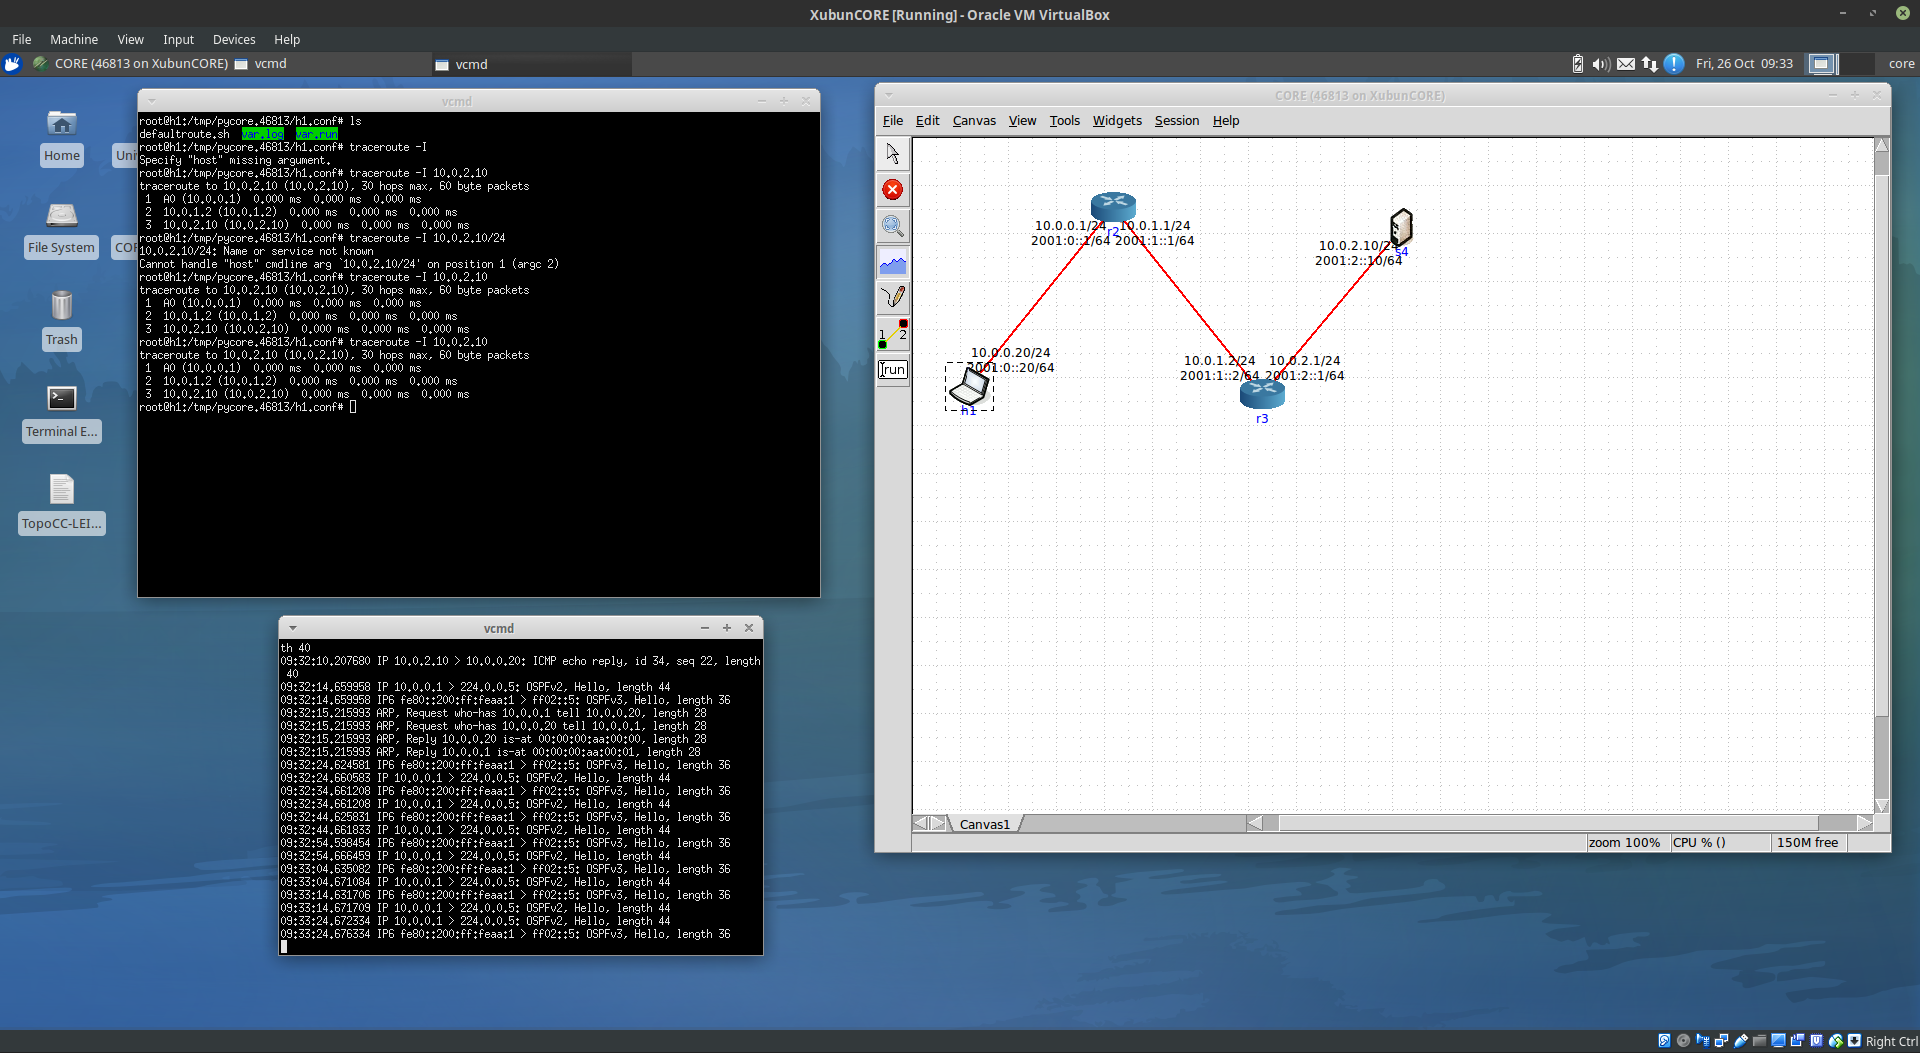
\includegraphics[scale=0.25]{pic1.png}\newline
    \caption{Topologia da rede (á direita), output do comando \textbf{traceroute -I} para s4 (em cima) e output do comando \textbf{tcdump} no pc h1 (em baixo).}
    \label{fig:my_label}
\end{figure}

\newpage

\textbf{--- b) Registe e analise o tráfego ICMP enviado por h1 e o tráfego ICMP recebido como resposta. Comento os resultados face ao comportamento.}\newline
\begin{figure}[!h]
    \centering
    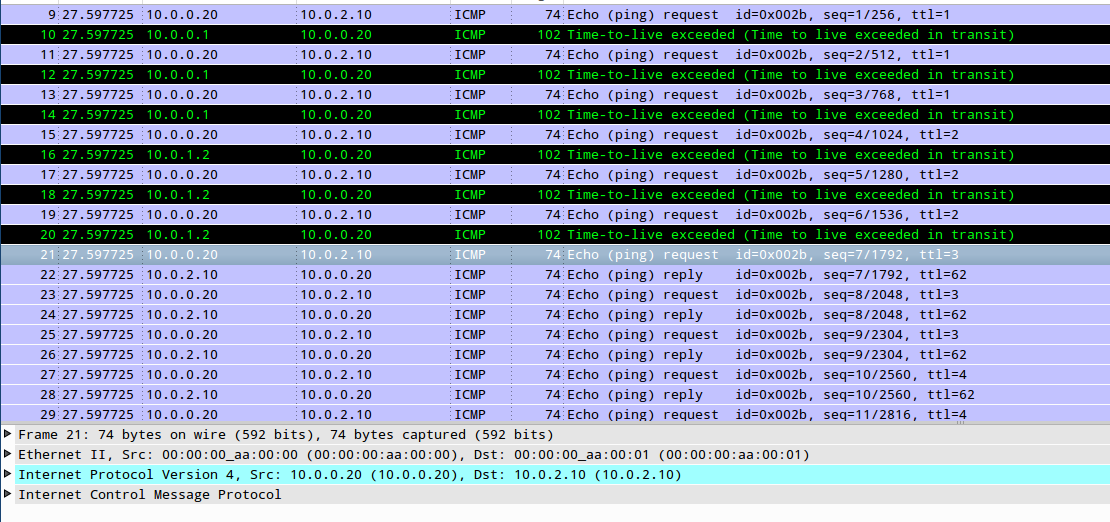
\includegraphics[scale=0.4]{parte2/2-b.png}\newline
    \caption{Primeiras mensagens ICMP enviadas pela nossa máquina.}
    \label{fig:my_label}
\end{figure}

O \textbf{traceroute} envia 3 mensagens ICMP com, inicialmente, o valor de TTL=1, e cada router por onde passa o pacote decrementa esta até chegar ao valor 0, onde envia uma resposta com \textit{Time-to-live exceeded}. À medida que vai falhando, envia novas mensagens com TTL superior ao anterior até encontrar um em que o pacote chegue ao destino sem que o TTL fique a 0, recebendo uma resposta \textit{Echo (ping)}. Assim, fica-se a saber quando saltos foram precisos para chegar ao destino (por quantos routers passou).\newline
Como podemos analisar na figura 2, enquanto o TLLT é inferior a 3 a nossa máquina recebe uma resposta \textit{Time-to-live exceeded}, sendo que apenas a partir de TTL igual ou superior a 3 é que recebe uma resposta \textit{Echo (ping)} - o pacote tem de passar por 3 routers antes de chegar ao destino.

\newpage

\textbf{--- c) Qual deve ser o valor inicial mínimo do campo TTL para alcançar o destino s4? Verifique na prtática que a sua resposta está correta.}\newline
O valor inicial mínimo do campo TTL para alcançar s4 é de 3.
\begin{figure}[ht]%
    \centering
    \subfloat[\textit{Wireshark} output para os vário TTL's.]{{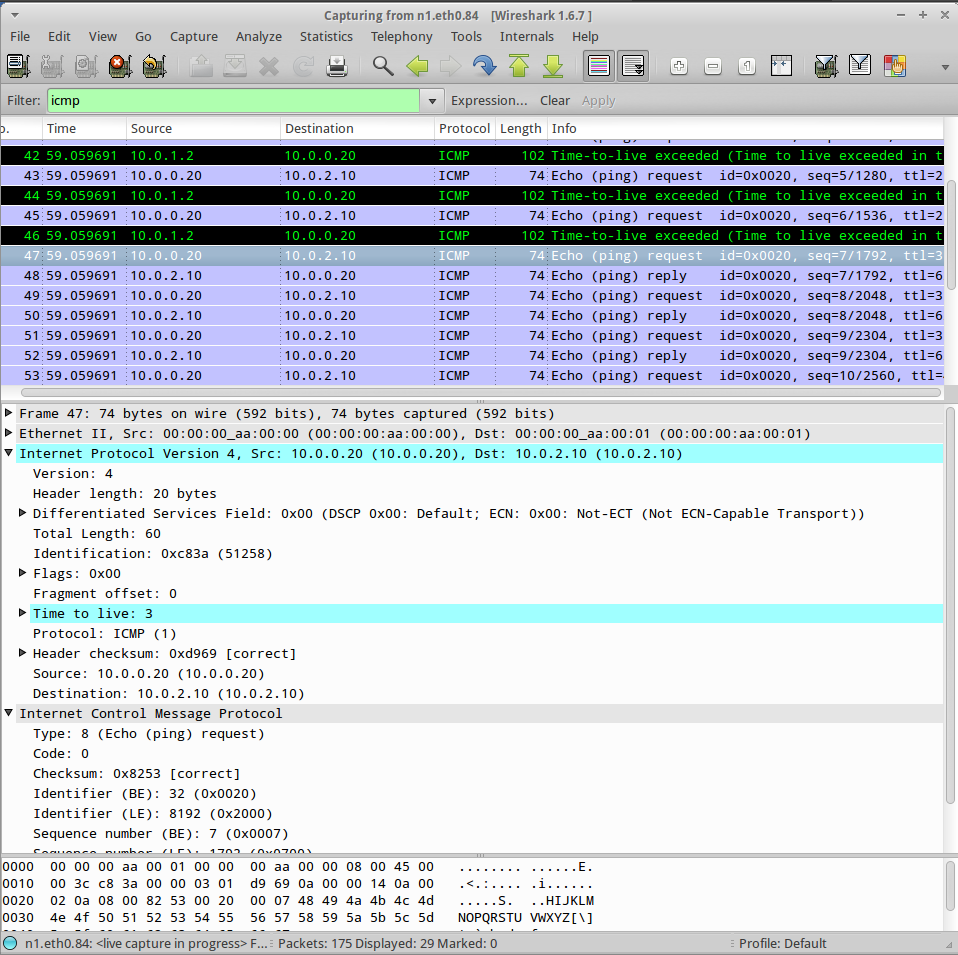
\includegraphics[width=7cm]{pic2-cropped.png}}}%
    \qquad
    \subfloat[Output de \textit{traceroute} com o número de saltos de h1 a s4.]{{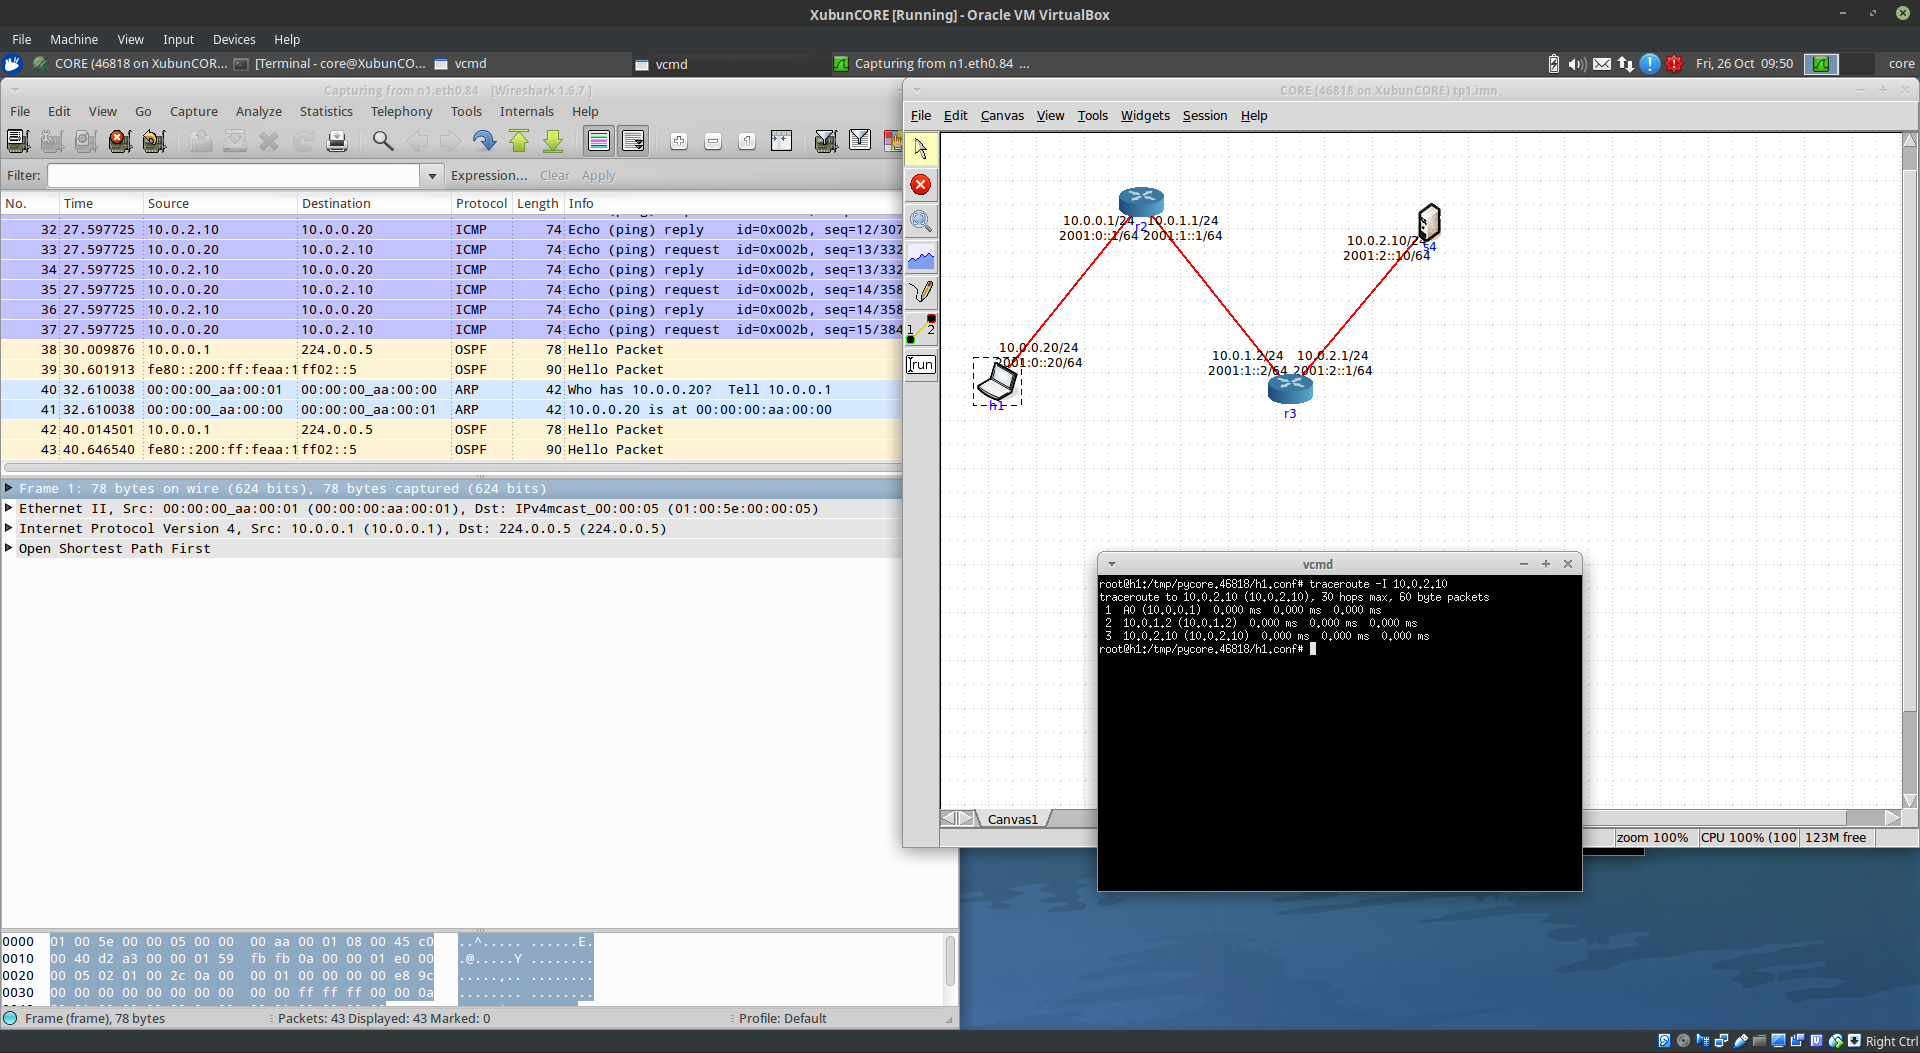
\includegraphics[width=7cm]{pic5.png}}}%
    \caption{Dois processos diferentes para descobrir o TTL mínimo para chegar a s4 a partir de h1.}%
    \label{fig:example}%
\end{figure}

Como se vê na figura a, só a partir do TTL\textgreater=3 é que há resposta do servidor. Através da figura b verificamos que, são precisos 3 \textit{hops} para chegar a s4.

\vspace{1cm}

\textbf{--- d) Qual o valor médio do tempo de ida-e-volta (Round-Trip Time) obtido?}\newline
Apesar de nos ter dado 0 de tempo médio, isto é impossivel pois claramente tem de existir uma demora entre o envio e a receção da resposta devido aos saltos e cálculos de routing executados por cada router até ao destino.
\begin{figure}[ht]
    \centering
    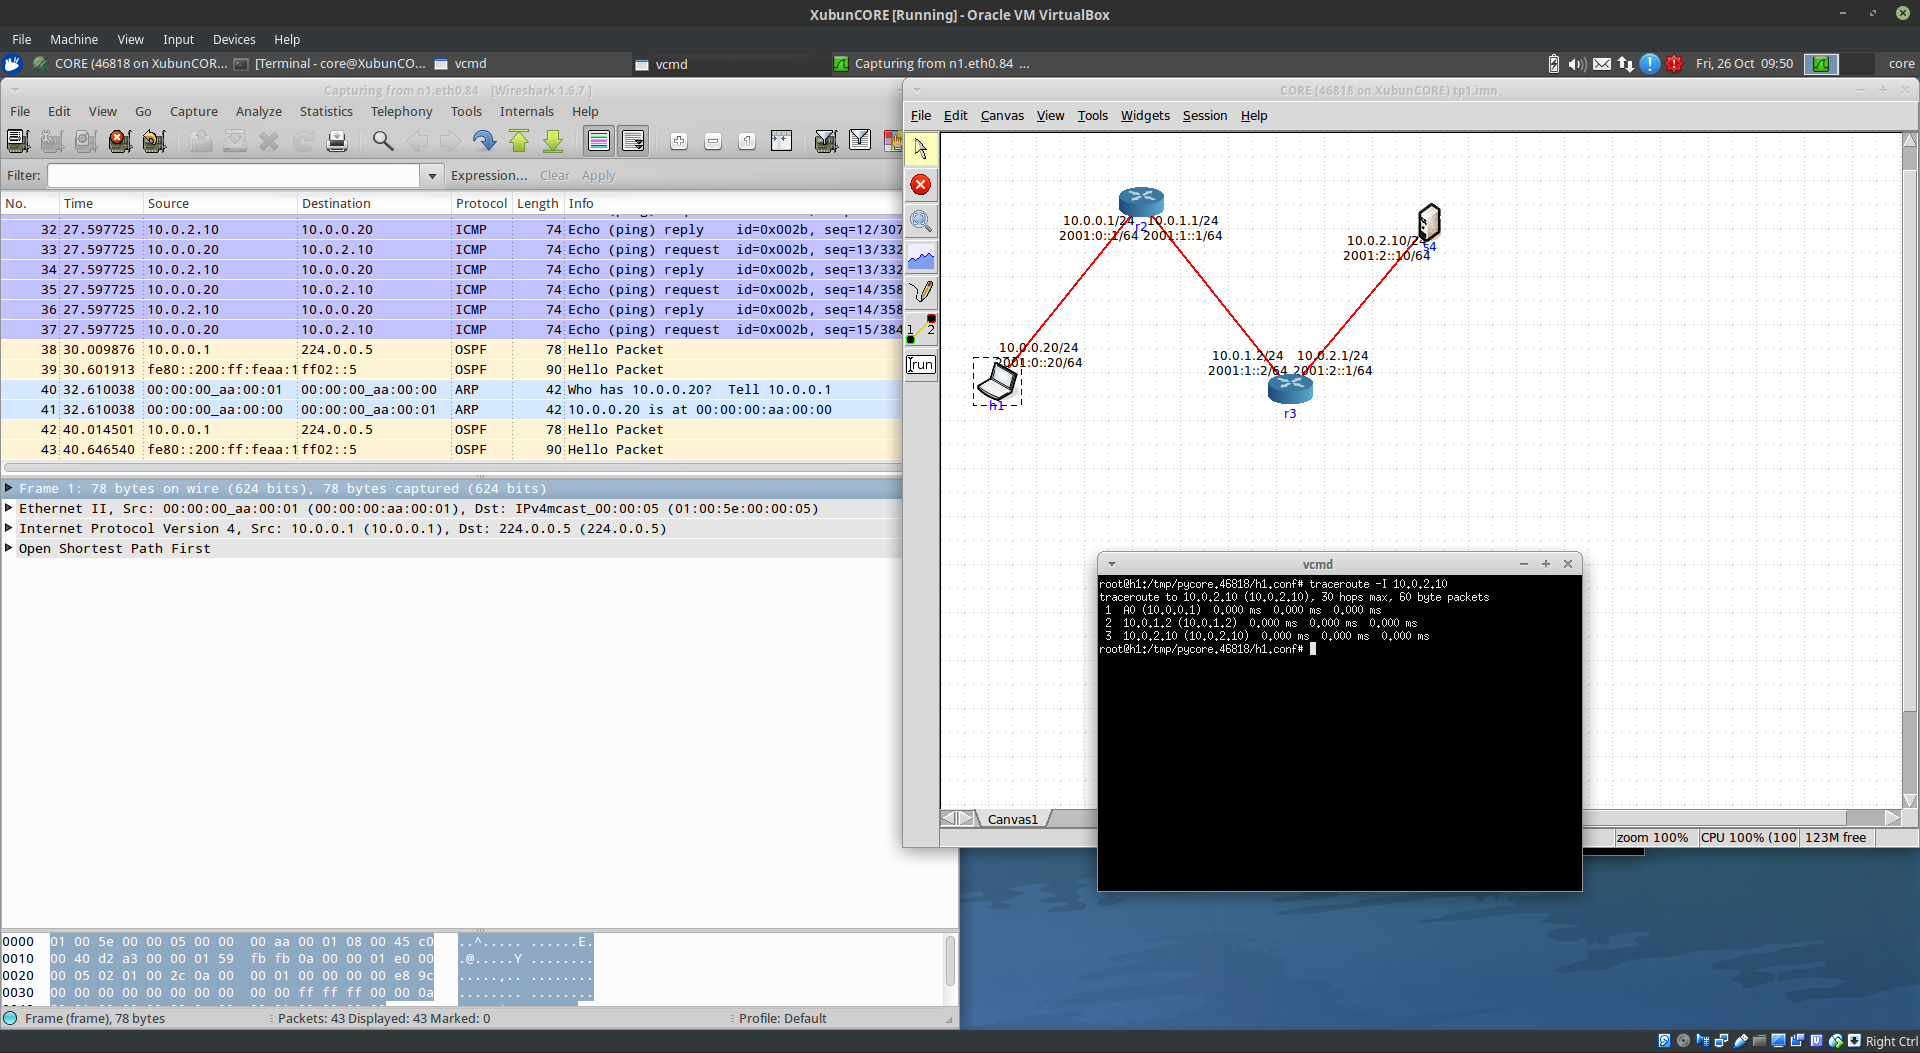
\includegraphics[scale=0.15]{pic5.png}
    \caption{Tempo médio de ida-e-volta entre h1 e s4.}

\end{figure}


\newpage


\textbf{2 - Procedimento a seguir:\newline
Usando o \textit{wireshark} capture o tráfego gerado pelo \textit{traceroute} para os seguintes tamanhos de pacote: (i) sem especificar, i.e., usando o tamanho por defeito; e (ii) 35XX bytes, em que XX é o seu número de grupo. Utilize como máquina destino o \textit{host} marco.uminho.pt. Pare a captura.}\newline
Com base no tráfego capturado, identifique os pedidos ICMP \textit{Echo Request} e o conjunto de mensagens devolvidas em resposta a esses pedidos.\newline
Selecione a primeira mensagem ICMP capturada (referente a (i) tamanho por defeito) e centre a análise no nível protocolar IP (expanda o \textit{tab} correspondente na janela de detalhe do \textit{wireshark}). Através da análise do cabeçalho IP diga:\newline
\vspace{1cm}

\textbf{--- a) Qual é o endereço IP da interface ativa do	seu	computador?}\newline
\begin{figure}[!htb]
    \centering
    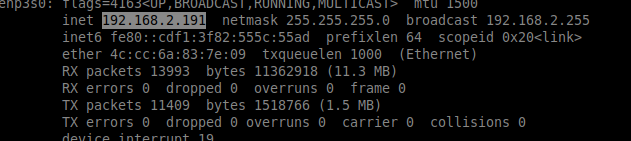
\includegraphics[scale=0.6]{pic7.png}\newline
    \caption{Endereço IP da interface Ethernet ligada á rede.}
    \label{fig:my_label}
\end{figure}
Usando o comando \textbf{ifconfig}, verificamos que o nosso IP é de 192.168.2.191.

\vspace{1cm}

\textbf{--- b) Qual é o valor do campo protocolo? O que identifica?}\newline
\begin{figure}[!htb]
    \centering
    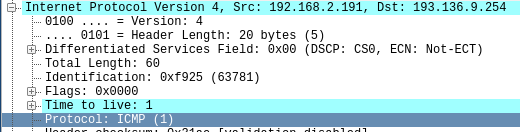
\includegraphics[scale=0.7]{valor-protocolo.png}\newline
    \caption{Detalhes do datagrama a nível do IP do datagrama em estudo capturado por \textit{wireshark}.}
    \label{fig:my_label}
\end{figure}
Como podemos ver na imagem, no nível do IP tem o campo protocolo com o valor 1 (ICMP). Identifica o protocolo ICMP (\textit{Internet Control Message Protocol}) usado pelo tráfego gerado pelo \textit{traceroute} para ajudar a mapear a rede.

\newpage

\textbf{--- c) Quantos \textit{bytes} tem o cabeçalho IP(v4)? Quantos \textit{bytes} tem o campo de dados (\textit{payload}) do datagrama? Como se calcula o tamanho do \textit{payload}?}\newline
\begin{figure}[ht]
    \centering
    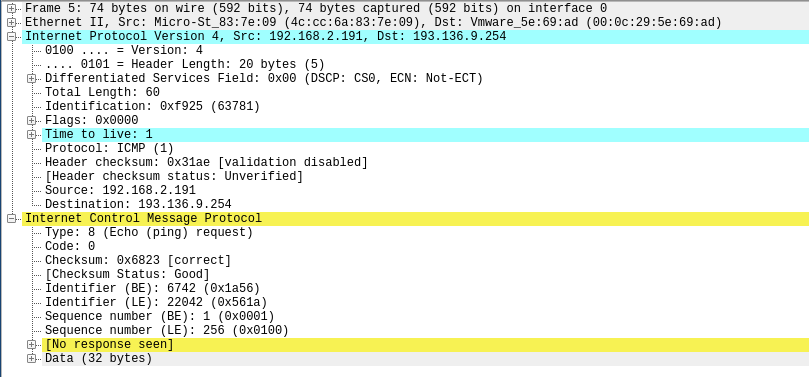
\includegraphics[scale=0.5]{datagrama-inicial.png}
    \caption{Detalhes do primeiro datagrama ICMP capturado pelo \textit{wireshark}.}
    \label{fig:my_label}
\end{figure}
Analizando o campo \textit{Header Length} concluimos que o cabeçalho tem 20 \textit{bytes}, o \textit{payload} tem 40 \textit{bytes} e calcula-se retirando ao tamanho total do datagrama o tamanho do cabeçalho: 60 - 20 = 40 \textit{bytes}. Apesar de parecer 40 \textit{bytes} de payload, na realidade são apenas 32 (como se verifica na figura). Os 8 \textit{bytes} em falta são utilizados no cabeçalho do protocolo UDP usado para transportar as mensagens ICMP.

\vspace{1cm}

\textbf{--- d) O datagrama IP foi fragmentado? Justifique.}\newline
\begin{figure}[!htb]
    \centering
    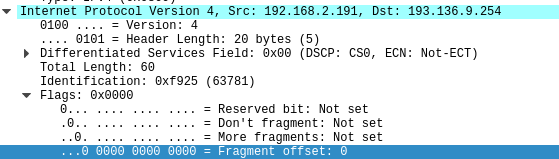
\includegraphics[scale=0.7]{pic9.png}\newline
    \caption{Campos referentes à fragmentação do datagrama em estudo.}
    \label{fig:my_label}
\end{figure}
O datagrama IP não foi fragmentado pois o valor de \textit{Fragment offset} é 0.

\newpage

\textbf{--- e) Ordene os pacotes capturados de acordo com o endereço IP fonte (e.g., selecionando o cabeçalho da coluna \textit{Source}), e analise a sequência de tráfego ICMP gerado a partir do endereço IP atribuído à interface da sua máquina. Para a sequência de mensagens ICMP enviadas pelo seu computador, identifique que campos do cabeçado IP variam de pacote para pacote.}\newline
\begin{figure}[h]%
    \centering
    \subfloat[Primeiro datagrama da lista.]{{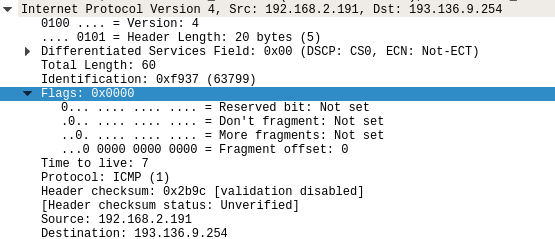
\includegraphics[width=7cm]{pic10cropped.png}}}%
    \qquad
    \subfloat[Segundo datagrama da lista.]{{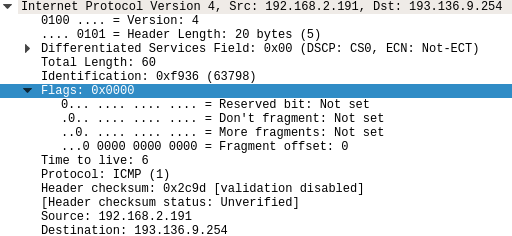
\includegraphics[width=7cm]{pic11.png}}}%
    \caption{Dois primeiros datagramas capturados.}%
    \label{fig:example}%
\end{figure}
Os campos que variam, analizando as imagens em cima apresentadas, são:
\begin{itemize}
    \item \textit{Identification}: campo que identifica o datagrama;
    \item \textit{Time to live}: campo com o número máximo de saltos que ainda podem ser feitos pelo datagrama. É usado para descobrir por quantos \textit{routers} passa um datagrama para ir de um dispositivo a outro;
    \item \textit{Header checksum}: Código de verificação do validade do datagrama (controlo de erros);
\end{itemize}

\vspace{1cm}

\textbf{--- f) Observa algum padrão nos valores do campo de Identificação do datagrama IP e TTL?}\newline
O valor de Identificação é imcrementado de 1 em 1 e o TTL é decrementado de 1 em 1 até chegar a 0.

\vspace{1cm}
\newpage

\textbf{--- g) Ordene o tráfego capturado por endereço destino e encontre a série de respostas ICMP TTL \textit{exceeded} enviadas ao seu computador. Qual é o valor do campo TTL? Esse valor permanece constante para todas as mensagens de resposta ICMP TTL \textit{exceeded} enviados ao seu \textit{host}? Porquê?}\newline
\begin{figure}[h]
    \centering
    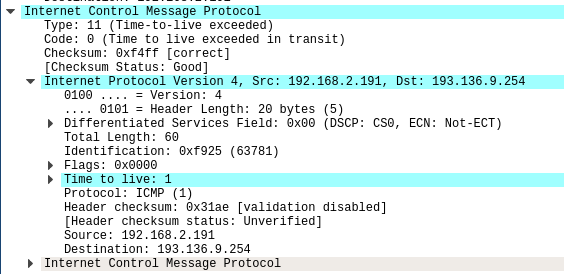
\includegraphics[scale=0.7]{pic12.png}
    \caption{Datagrama de uma resposta ICMP com TTL \textit{exceeded}.}
    \label{fig:my_label}
\end{figure}
O valor do campo TTL é 1 e permanece constante, pois se ocorreu TTL \textit{exceeded} significa que o pacote não consegui chegar ao destino, tendo sido um router o último a decrementar o TLL, indo para 0, descartando este e enviando uma mensagem de erro (Time-to-live exceeded).

\vspace{1cm}
\clearpage

\textbf{3 - Pretende-se agora analisar a fragmentação de pacotes IP. Reponha a ordem do tráfego capturado usando a coluna do tempo de captura. Observe o trávego depois do tamanho de pacote ter sido definido para 35XX \textit{bytes}.}\newline
\vspace{1cm}

\textbf{--- a) Localize a primeira mensagem ICMP. Porque é que houve necessidade de fragmentar o pacote inicial?}\newline
Houve necessidade de fragmentar o pacote porque o seu tamanho excedia o MTU (\textit{Maximum Transmission Unit}) de 1500 (como nós enviamos um pacote com 3556 \textit{bytes} e o primeiro fragmento tem 1500 de tamanho, deduz-se que o MTU seja de 1500).

\vspace{1cm}

\textbf{--- b) Imprima o primeiro fragmento do datagrama IP segmentado. Que informação no cabeçalho indica que o datagrama foi fragmentado? Que informação no cabeçalho IP indica que se trata do primeiro fragmento? Há mais fragmentos? Qual é o tamanho deste datagrama IP?}\newline
\begin{figure}[!htb]
    \centering
    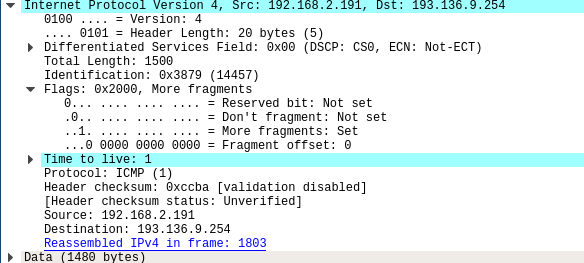
\includegraphics[scale=0.7]{pic13.png}\newline
    \caption{Detalhes do primeiro fragmento do datagrama em estudo.}
    \label{fig:my_label}
\end{figure}

O campo \textit{More Fragments} indica que existem mais fragmentos desta mensagem. Como o \textit{Fragment offset} é igual a 0, significa que este é o primeiro fragmento e tem o tamanho de 1500 \textit{bytes}, sendo o tamanho total do datagrama de 3556.

\vspace{1cm}
\newpage

\textbf{--- c) Imprima o segundo fragmento do datagrama IP original. Que informação do cabeçalho IP indica que não se trata do 1º fragmento? Há mais fragmentos? O que nos permite afirmar isso?}\newline
\begin{figure}[!htb]
    \centering
    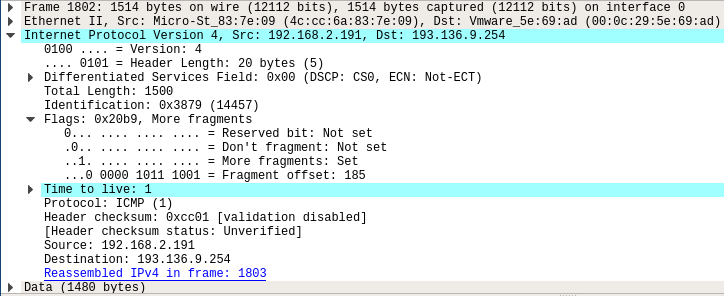
\includegraphics[scale=0.6]{pic14.png}\newline
    \caption{Detalhes do segundo fragmento do datagrama em estudo.}
    \label{fig:my_label}
\end{figure}
Podemos identificar que não se trata do primeiro fragmento através do campo \textit{Fragment offset} e existem mais fragmentos pois o campo \textit{More fragments} está a 1.

\vspace{1cm}

\textbf{--- d) Quantos fragmentos foram criados a partir do datagrama orginal? Como se detecta o último fragmento correspondente ao datagrama original?}\newline
\begin{figure}[!htb]
    \centering
    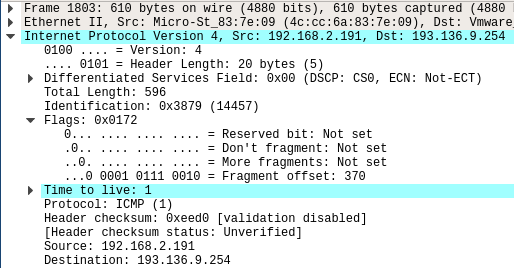
\includegraphics[scale=0.7]{pic15.png}\newline
    \caption{Detalhes do terceiro (e último) fragmento do datagrama em estudo.}
    \label{fig:my_label}
\end{figure}
Foram criados 3 fragmentos a partir do datagrama original e o último é idetificado pelo campo \textit{More Fragments} a 0 e possuindo um \textit{Fragment offset} maior que o anterior fragmento.\newline
Neste datagrama em particular, podemos verificar que este último fragmento possui um tamanho inferior a todos os outros, podendo então afirmar que é, de facto, o último.


\textbf{--- e) Indique, resumindo, os campos que mudam no cabeçalho IP entre os diferentes fragmentos, e explique a forma como essa informação permite reconstruir o datagrama original.}\newline
Os campos que mudam no cabeçalho IP são os seguintes (usando as figuras 11, 12 e 13 para comparação):
\begin{itemize}
    \item Flags: o campo \textit{More fragments} fica a 1 até se chegar ao último fragmento e o \textit{Fragment offset} vai aumentando por fragmento;
    \item \textit{Header checksum}: este muda pois a simples alteração de um campo no cabeçalho origina um código de validação diferente;
    \item \textit{Total Length}: apenas o último fragmento poderá ter um tamanho inferior aos restantes fragmentos.
\end{itemize}
A reconstrução é possível através de dois importantes aspectos do cabeçalho: identificação e \textit{Fragment offset}. Com a identificação agregamos os datagramas que possuem este valor igual entre si, ficando assim apenas aqueles fragmentos que pertencem ao datagrama original. Depois, usando o \textit{Fragment offset}, 
ordenamos os fragmentos por ordem crescente do \textit{offset}, ficando assim com a ordem correta dos fragmentos.


\newpage

\subsection{2ª Parte}
Caso de estudo: Considere que a organização MIEI-RC é constituída por três departamentos(A,B e C) e cada
departamento possui um \textit{router} de acesso à sua rede local. Estes \textit{routers} de acesso (Ra, Rb e Rc) estão
interligados entre si por ligações Ethernet a 1Gbps, formando um anel. Por sua vez, existe um servidor (S1) na rede do departamento C e, pelo menos, três \textit{laptops} por departamento, interligados ao \textit{router} respetivo através de um comutador (\textit{switch}). S1 tem uma ligação a 1Gbps e os \textit{laptops} ligações a 100Mbps. Considere apenas a existência de um comutador por departamento.\newline
A conectividade IP externa da organização é assegurada através de um router de acesso Rext conectado a Rc por uma ligação ponto-a-ponto a 10 Gbps.\newline
Construa uma tolopogia CORE que reflita a rede local da empresa. Para facilitar a visualização pode ocultar o endereçamento IPV6.\newline

\textbf{1 - Atenda aos endereços IP atribuídos automaticamente pelo CORE aos diversos equipamentos da topologia.}\newline
\vspace{1cm}

\textbf{--- a) Indique que endereços IP e máscaras de rede foram atribuídos pelo CORE a cada equipamento. Para simplificar, pode incluir uma imagem que ilustre de forma clara a topologia definida e o endereçamento usado.}\newline
\begin{figure}[h]
    \centering
    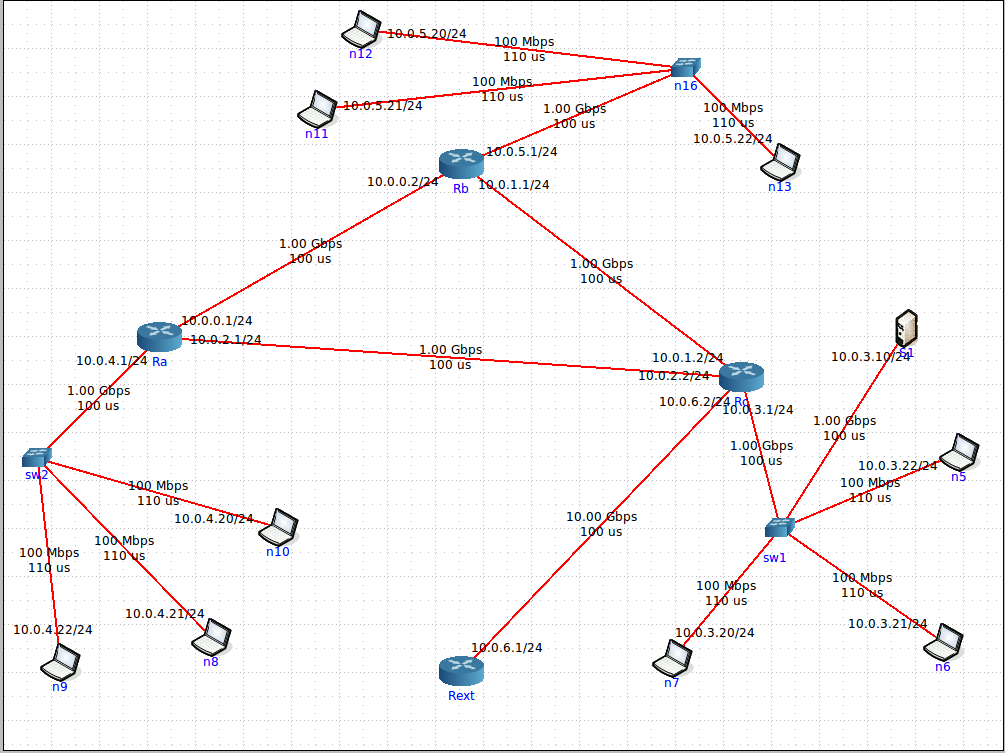
\includegraphics[scale=0.3]{parte2/topologia.png}\newline
    \caption{Topologia da rede em estudo.}
    \label{fig:my_label}
\end{figure}
\clearpage
Cada equipamento possui os IP's visiveis na figura. Existem 7 sub-redes atribuidas (com máscara de 255.255.255.0):
\begin{itemize}
    \item 10.0.0.0/24
    \item 10.0.1.0/24
    \item 10.0.2.0/24
    \item 10.0.3.0/24
    \item 10.0.4.0/24
    \item 10.0.5.0/24
    \item 10.0.6.0/24
\end{itemize}

\vspace{1cm}

\textbf{--- b) Tratam-se de endereços públicos ou privados? Porquê?}\newline
Tratam-se de endereços privados pois pertencem á gama 10.0.0.0/8, uma gama standard de redes privadas.

\vspace{1cm}

\textbf{--- c) Porque razão não é atribuído um endereço IP aos \textit{switches}?}\newline
Não  são atribuídos IPs aos \textit{switches} pois estes são dispositivos de 2ªcamada (\textit{data link layer}), não possuindo IPs (embora possam existir com a 3ª camada (\textit{network layer}) como um router).


\newpage
\textbf{--- d) Usando o comando \textbf{ping} certifique-se que existe conectividade IP entre os \textit{laptops} dos vários departamentos e o servidor do departamento C (basta certificar-se da conectividade de um \textit{laptop} por departamento).}\newline
\begin{figure}[h]%
    \centering
    \subfloat[Conectividade entre \textit{laptop} de Ra e servidor S1]{{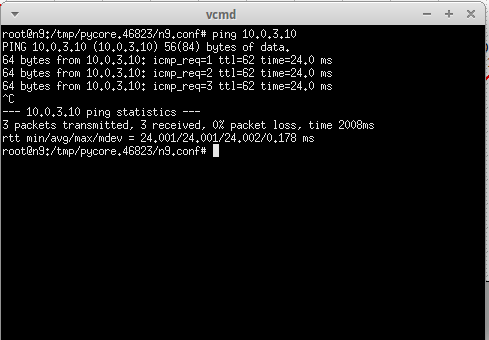
\includegraphics[width=7cm]{parte2/ra-s1.png}}}%
    \qquad
    \subfloat[Conectividade entre \textit{laptop} de Rb e servidor S1]{{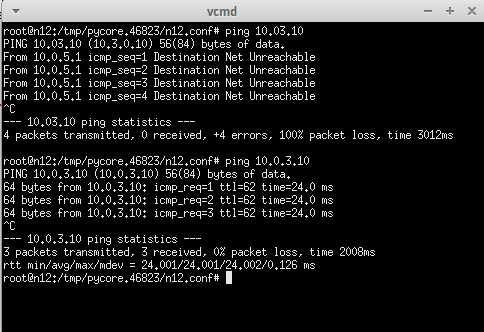
\includegraphics[width=7cm]{parte2/rb-s1.png}}}%
    \qquad
    \subfloat[Conectividade entre \textit{laptop} de Rc e servidor S1]{{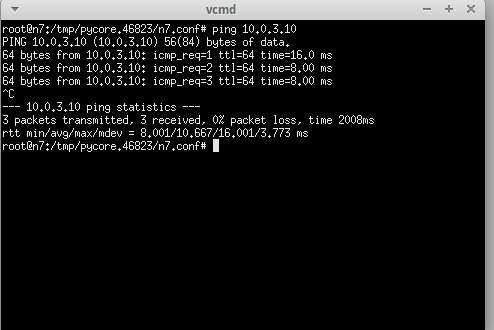
\includegraphics[width=7cm]{parte2/rc-s1.png}}}%
    \caption{Prova de conectividade entre os \textit{laptop} dos diferentes departamentos e o servidor do departamento C}%
    \label{fig:example}%
\end{figure}

\newpage

\textbf{--- e) Verifique se existe conectividade IP do router de acesso Rext para o servidor S1.}\newline
\begin{figure}[h]
    \centering
    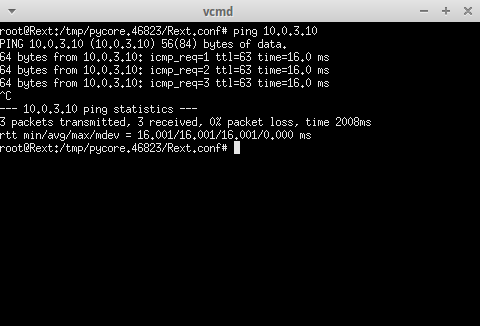
\includegraphics[scale=1]{parte2/rext-s1.png}\newline
    \caption{Conectividade IP entre router de acesso Rext e o servidor S1}
    \label{fig:my_label}
\end{figure}

\newpage

\textbf{2 - Para o router e um \textit{laptop} do departamento A:}\newline

\textbf{-- a) Execute o comando \textbf{netstat -rn} por forma a poder consultar a tabela de enchaminhamento unicast (IPv4). Inclua no seu relatório as tabelas de encaminhamento obtidas; interprete as várias entradas de cada tabela. Se necessário, consulte o manual respetivo (\textbf{man netstat}).}\newline

\underline{Extra info:}
\begin{itemize}
    \item Flag U: Informa que a rota está válida.
    \item Flag G: Informa que \textit{gateway} é um router para depois ser reencaminhado por este (não está ligado diretamente ao IP destino).
\end{itemize}

\begin{figure}[!htb]
    \centering
    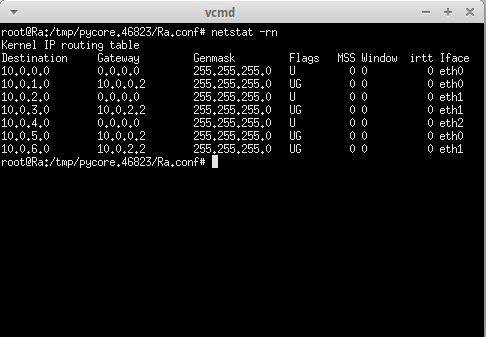
\includegraphics[scale=1]{parte2/tabela-routerA.png}\newline
    \caption{Tabela de encaminhamento do router Ra}
    \label{fig:my_label}
\end{figure}
Na tabela do router verificamos as seguintes 7 entradas:
\begin{itemize}
    \item 10.0.0.0 $\rightarrow$ 0.0.0.0 : Define que tráfego enviado para um IP destino dentro da sub-rede (10.0.0.0/24) seja encaminhado diretamente para o equipamento sem ter de passar pelo router (estão ligados fisicamente).
    \item 10.0.1.0 $\rightarrow$ 10.0.0.2: Esta entrada define que o tráfego enviado para qualquer IP de 10.0.1.0/24 seja enviado para o router em 10.0.0.2 (router Rb) para depois este reencaminhar.
    \item 10.0.2.0 $\rightarrow$ 0.0.0.0: O tráfego enviado pra qualquer IP da sub-rede 10.0.2.0/24 é enviado diretamente para o equipamento destino, pois estão ligado fisicamente na mesma sub-rede.
    \item 10.0.3.0 $\rightarrow$ 10.0.2.2: Define que o tráfego enviado para qualquer IP de 10.0.3.0/24 seja enviado para o router em 10.0.2.2 (router Rc) para depois este reencaminhar.
    \item 10.0.4.0 $\rightarrow$ 0.0.0.0: O tráfego enviado pra qualquer IP da sub-rede 10.0.4.0/24 é enviado diretamente para o equipamento destino, pois estão ligado fisicamente na mesma sub-rede.
    \item 10.0.5.0 $\rightarrow$ 10.0.0.2: Esta entrada define que o tráfego enviado para qualquer IP de 10.0.5.0/24 seja enviado para o router em 10.0.0.2 (router Rb) para depois este reencaminhar.
    \item 10.0.6.0 $\rightarrow$ 10.0.2.2: O tráfego enviado para qualquer IP de 10.0.6.0/24 seja enviado para o router em 10.0.0.2 (router Rc) para depois este reencaminhar.
\end{itemize}


\begin{figure}[!htb]
    \centering
    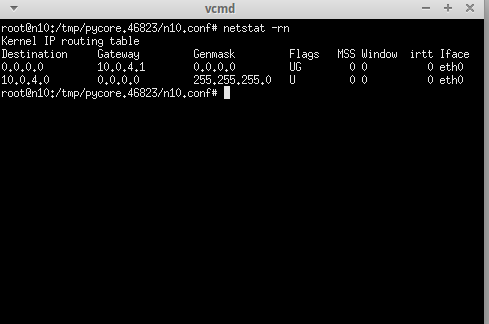
\includegraphics[scale=1]{parte2/laptop-tabela.png}\newline
    \caption{Tabela de encaminhamento do \textit{laptop} 10 (n10)}
    \label{fig:my_label}
\end{figure}
Nesta tabela podemos verificar que tem duas entradas:
\begin{itemize}
    \item 0.0.0.0 $\rightarrow$ 10.0.4.1: Esta entrada define que tráfego para qualquer IP de destino seja reencaminhado para o router Ra (10.0.4.1) que depois terá a função de continuar o encaminhamento até ao destino final.
    \item 10.0.4.0 $\rightarrow$ 0.0.0.0: Esta entrada define que o tráfego enviado para um IP destino dentro da sub-rede (10.0.4.0/24) seja encaminhado diretamente para o equipamento sem ter de passar pelo router  (estão ligados fisicamente).
\end{itemize}

\textbf{-- b) Diga, justificando, se está a ser usado encaminhamento estático ou dinâmico (sugestão: analise que processos estão a correr em cada sistema).}\newline
Usando o comando \textbf{ps -e} em ambos um router e um \textit{laptop}, verificamos que:
\begin{itemize}
    \item Router: existe um processo a correr chamdo \textit{ospfd} que é um software the encaminhamento dinâmmico;
    \item \textit{Laptop}: não existe nenhum processo referente a qualquer tipo de software the encaminhamento dinâmico, logo é estático.
\end{itemize}

\begin{figure}[!htb]
    \centering
    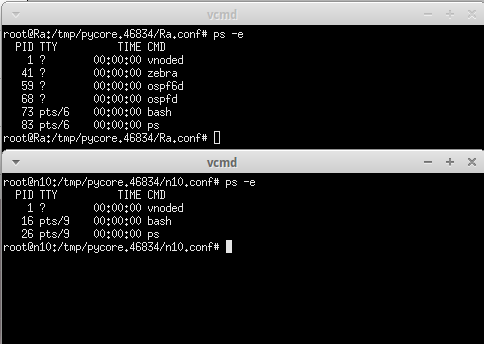
\includegraphics[scale=1]{parte2/processos.png}\newline
    \caption{Lista de processos a decorrer no router Ra.}
    \label{fig:my_label}
\end{figure}

\newpage

\textbf{--- c) Admita que, por questões administrativas, a rota por defeito (0.0.0.0 ou \textit{default}) deve ser retirada da tabela de encaminhamento do servidor S1 localizado no departamento C. Use o comando \textbf{route delete} para o efeito. Que implicações tem esta medida para os utilizadores da empresa que acedem ao servidor? Justifique.}\newline
Os utlizadores deixam de puder comunicar com o servidor, pois este não consegue comunicar com redes externas à sua sub-rede - não sabe o que fazer com IP's fora da sua sub-rede). Este apenas consegue comunicar com os dispositivos a que está ligado fisicamente (na mesma sub-rede).
\begin{figure}[h]
    \centering
    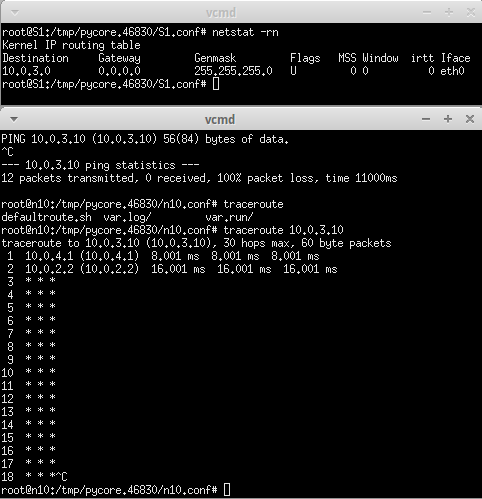
\includegraphics[scale=1]{parte2/notconnected.PNG}\newline
    \caption{Servidor S1 não acessível por um \textit{laptop} fora da sua sub-rede.}
    \label{fig:my_label}
\end{figure}

\vspace{1cm}

\textbf{--- d) Adicione as rotas estáticas necessárias para restaurar a conectividade para o servidor S1, por forma a contornar a restrição imposta na alínea c). Utilize para o efeito o comando \textbf{route add} e registe os comandos que usou.}\newline
Comandos usados:
\begin{itemize}
    \item route add -net 10.0.4.0 netmask 255.255.255.0 gw 10.0.3.1
    \item route add -net 10.0.5.0 netmask 255.255.255.0 gw 10.0.3.1
\end{itemize}


\textbf{--- e) Teste a nova política de encaminhamento garantido que o servidor está novamente acessível, utilizando para o efeito o comando \textbf{ping}. Registe a nova tabela de encaminhamento do servidor.}\newline
\begin{figure}[!htb]
    \centering
    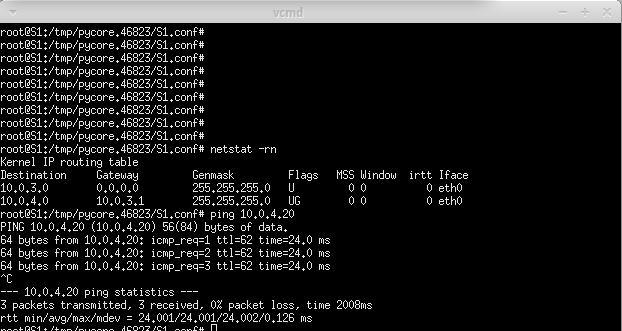
\includegraphics[scale=0.7]{parte2/nova-tabela-de-encaminhamento.png}\newline
    \caption{Prova de conectividade entre um computador da sub-rede 10.0.4.0/24 (especificamento do equipamento 10.0.4.20) e o servidor S1, com a nova rota definida.}
    \label{fig:my_label}
\end{figure}
\begin{figure}[!htb]
    \centering
    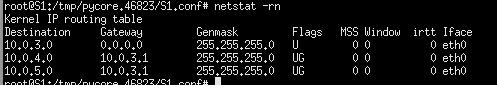
\includegraphics[scale=1]{parte2/nova-tabela.png}\newline
    \caption{Nova Tabela de encaminhamento do servidor S1.}
    \label{fig:my_label}
\end{figure}

\newpage

\textbf{3 - Por forma a minimizar a falta de endereços IPv4 é comum a utilização de sub-redes. Além disso, a definição de sub-redes permite uma melhor organização do espaço de endereçamento das redes em questão.\newline
Para definir endereços de sub-rede é necessário usar a parte prevista para endereçamento de \textit{host}, não sendo possível alterar o endereço de rede original. Recorda-se que o \textit{sub-redeting}, ao recorrer ao espaço de endereçamento para \textit{host}, implica que possam ser endereçados menos \textit{hosts}.}\newline
Considere a topologia definida anteriormente. Assuma que o endereçamento entre os \textit{routers} se mantém inalterado, contudo, o endereçamento em cada departamento deve ser redefinido.

\vspace{1cm}

\textbf{--- a) Considere que dispõe apenas do endereço de rede IP 172.XX.48.0/20, em que XX é o decimal correspondendo ao seu número de grupo (PLXX). Defina um novo esquema de endereçamento para as redes dos departamentos (mantendo a rede de acesso e core inalteradas) e atribua endereços às interfaces dos vários sistemas envolvidos. Deve justificar as opções usadas.}\newline

Como são apenas 3 departamentos, para possibilitar a expansão destes e melhor organização da rede destes, definimos 3bits para sub-rede, tornando-se a máscara de rede /23.
Sendo que dispomos do endereço IP 172.56.48.0/20, criamos o seguinte esquema:

\begin{table}[h]
\begin{tabular}{|l|l|l|l|l|}
\hline
SA & 172.56.48.0/23 & 172.56.49.0/23 & 510 hosts & Departamento A \\ \hline
SB & 172.56.50.0/23 & 172.56.51.0/23 & 510 hosts & Departamento A \\ \hline
SC & 172.56.52.0/23 & 172.56.53.0/23 & 510 hosts & Departamento B \\ \hline
SD & 172.56.54.0/23 & 172.56.55.0/23 & 510 hosts & Departamento B \\ \hline
SE & 172.56.56.0/23 & 172.56.57.0/23 & 510 hosts & Departamento C \\ \hline
SF & 172.56.58.0/23 & 172.56.59.0/23 & 510 hosts & Departamento C \\ \hline
SG & 172.56.60.0/23 & 172.56.61.0/23 & 510 hosts & Outros            \\ \hline
SH & 172.56.62.0/23 & 172.56.63.0/23 & 510 hosts & Outros            \\ \hline
\end{tabular}
\end{table}

\underline{Nota}: não retiramos a primeira e última sub-redes, pois apesarem de estas terem sido reservadas no passado, atualmente osrouters modernos têm a capacidade de os usarem.

Assim, o departamento A ficará com SA e, caso queira expandir e para facilitar, com a gama de SB, o departamento B com SC e SD e o departamento C com SE e SF.\newline
Mas é importante referir que a organização da rede depende muito do cenário em que será aplicado, sendo este um cenário imaginado por nós onde se aplique esta determinada organização.

\vspace{1cm}

\textbf{--- b) Qual a máscara de rede que usou (em formato decimal)? Quantos \textit{hosts} IP pode interligar em cada departamento? Justifique.}\newline
A máscara de rede usada foi /23, ou seja, 255.255.254.0, criando 8 sub-redes, podendo cada departamento pode interligar 510 \textit{hosts}. Optamos por esta escolha, visto que, com 8 sub-redes permite a cada departamento (três por agora) usar até duas gamas de IPs, sobrando ainda outras duas para uma possível adição de uma outra sub-rede. Assim, cada departamento pode usar um máximo de 1020 \textit{hosts} caso use as suas duas sub-redes respectivas.

\newpage

\textbf{--- c) Garanta e verifque que conectividade IP entre as várias redes locais da organização MIEI-RC é mantida. Explique como procedeu.}\newline
A cada departamento atribuimos IP's da gama da sua sub-rede e para testar conectividade usamos o comando \textbf{ping} com o IP de máquinas de outras sub-redes.
\begin{figure}[h]
    \centering
    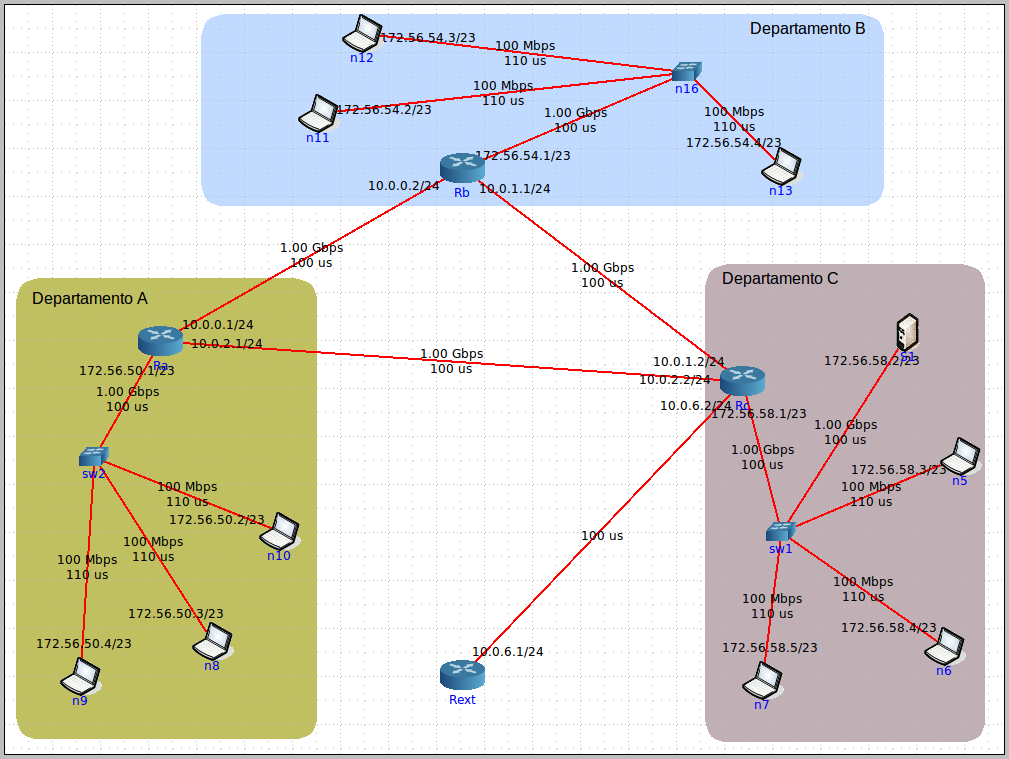
\includegraphics[scale=0.5]{parte2/nova-topo-cores.png}\newline
    \caption{Nova Topologia da rede em estudo.}
    \label{fig:my_label}
\end{figure}
\begin{figure}[h]
    \centering
    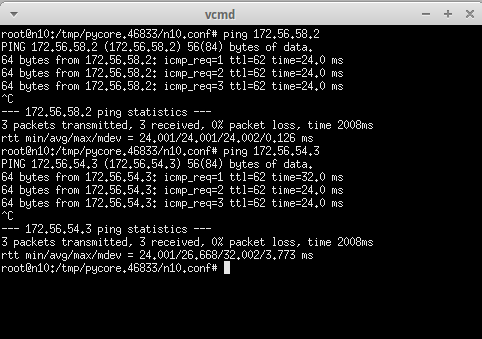
\includegraphics[scale=1]{parte2/ping-nova-topologia.png}\newline
    \caption{Prova de conectividade entre as diferentes sub-redes: n10 (Dep A) e S1 (Dep C); n10 (Dep A) e n11 (Dep B).}
    \label{fig:my_label}
\end{figure}


\vspace{5cm}

\section{Conclusões}

Com a resolução deste trabalho foi possível abordar as temáticas da Unidade Curricular de Redes e Computadores de forma mais aprofundada, consolidando o conhecimento adquirido nas aulas teóricas. 
 A primeira secção teve como foco principal o protocolo IPv4 com especial atenção  nos datagramas IP e na fragmentação incluídos. Através da utilização da tecnologia \textit{Core} foi possível representar topologias de redes e desta forma analisar como os pactotes se comportam nas redes. Numa primeira abordagem foi analisado o TTL e do quão importante é ter um TTL baixo para que os pacotes cheguem rapidamente ao seu destino. Para análise do TTL foi necessária a ferramenta \textit{Wireshark} que mostra aos utilizadores os pacotes que estão em movimento na rede. Ainda nesta seccção foi explorado como o protocolo ICMP é incluído no pacote (através da utilização de um header), o tamanho que este ocupa bem como o que verdadeiramente é a informação que se pretende transmitir. Podemos também analizar e entender como se processa a fragmentação de um pacote, que ocorre quando não é possível enviar a informação todo num pacote e se tem de enviar em vários, e de como os pacotes se identificavam entre si.\newpage
 
 A segunda secção, embora ainda dedicada ao protocolo IPv4, teve como temáticas o endereçamento e encaminhamento IP. Para isso foi utilizado novamente o \textit{Core} para representar uma toplologia de vários departamentos. Foi desta forma analizada se os IP's da topologia eram privados ou públicos e a razão pela qual diferentes computadores conseguem comunicar entre diferentes sub-redes utilizando routers. Quanto ao endereçamento foi verificado se o encaminhamento era estático ou dinâmico podendo assim assimilar os conceitos que aparentam ser mais teóricos de uma forma mais aproximada à realidade, concluindo que nos dias de hoje, nas tecnologias usadas os routers são bastante inteligentes e fazem um encaminhamento dinâmico para máxima eficiência.\newline
 
 Foi também percebido a importância de uma boa organização da rede, para melhor utilização do espaço de endereçamento associado a esta - tudo dependendo da utilização final e futuras expansões desta mesma. A criação de sub-redes, a atribuição destas a diferentes zonas da rede e o processo de encaminhamento, foram todos importantes aspetos estudados e bem assimilados.
\end{document}
